\section{Does the Qualified Design Pay? (RQ3)}
\label{sec:cost}
\subsection{RTX: deployment gain and speculative increment}
The RTX expansion measures four conditions in four balanced rounds. Ordinary $R$ uses mask 0/UB1 without draft; matched $M$ uses mask 3/UB4 without draft; candidate $C$ (also denoted $C_3$) uses mask 3/UB4/$k=3$; $C_{15}$ uses mask 15. Each round has four separate resident processes, each with one excluded warmup and 24 formal requests. Condition and task orders rotate; recorded cache reuse is zero. Thus the paths share a panel and campaign but not one simultaneous resident process.

Table~\ref{tab:rtx_cost} reports the same-record CPU reconstruction against both paid baselines. Generation speed is $1.170124\times$ ordinary and $1.169238\times$ matched execution, with 22/24 tasks faster in each comparison. Resident-request speed is $1.741569\times$ ordinary but $1.035071\times$ matched. Crucially, $R/M$ request speed is $1.682560\times$: most of the ordinary-reference request improvement is available without speculation. The $1.742\times$ result is the benefit of the full deployment change and cannot be assigned entirely to speculative execution.

% Generated by scripts/reconstruct.py from frozen exports.
\begin{table}[ht]\centering\small
\caption{RTX frozen expansion paid ratios: 24 task medians, four repeats. Gen. denotes generation; Request denotes resident request. Intervals describe task resampling. $C_3$ is mask 3 speculation.}\label{tab:rtx_cost}
\setlength{\tabcolsep}{4pt}
\begin{tabular}{@{}llrr@{}}\toprule
Ratio & Timer & Speed & 95\% interval\\\midrule
$R$/$C_3$ & Gen. & 1.170 & [1.117,1.218]\\
$R$/$C_3$ & Request & 1.742 & [1.655,1.827]\\
$M$/$C_3$ & Gen. & 1.169 & [1.117,1.217]\\
$M$/$C_3$ & Request & 1.035 & [1.005,1.063]\\
$R$/$M$ & Gen. & 1.001 & [0.995,1.008]\\
$R$/$M$ & Request & 1.683 & [1.590,1.766]\\
\bottomrule\end{tabular}

\end{table}


Figure~\ref{fig:cost} separates comparator construction from the three measured ratios, keeping generation and resident-request intervals distinct. All 48 task-level timer identities and both aggregate identities satisfy Equation~\ref{eq:identity}; this check does not provide a component-cost profile.

\begin{figure*}[t]
\centering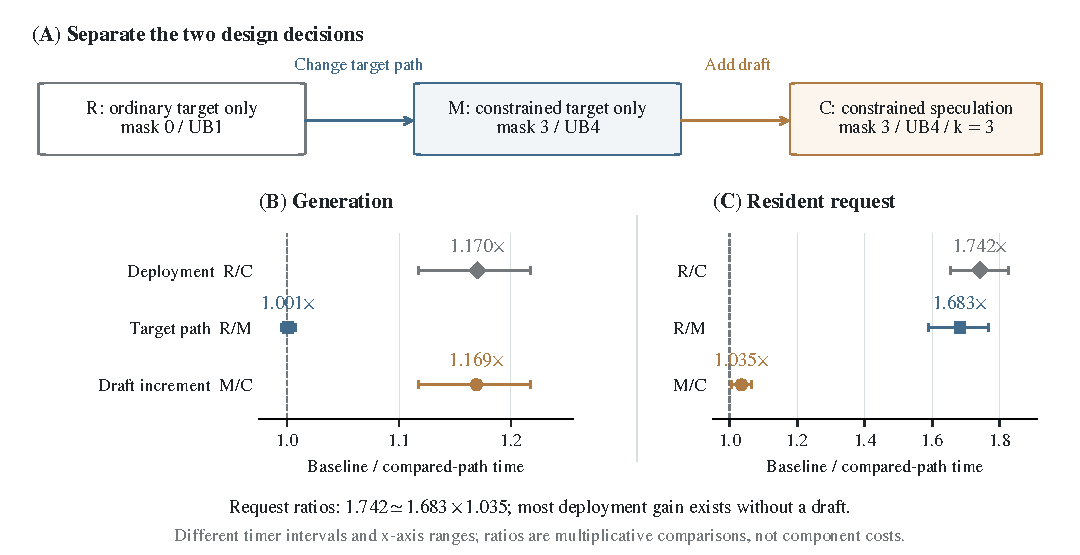
\includegraphics[width=\linewidth]{figures/figure_4_paid_cost.pdf}
\caption{Check the comparator before attributing a speedup. (A) Ordinary $R$, matched draft-free $M$, and mask-3 speculative $C$ distinguish the target-path change from the addition of a draft. (B,C) Geometric-mean ratios of 24 task medians from four repetitions; bars are descriptive 95\% task-bootstrap intervals. The two timer domains and x-axis ranges differ. The request-ratio identity is multiplicative and does not decompose component costs. A ratio above one favors the denominator path.}
\label{fig:cost}
\end{figure*}

The target-path comparison changes prefill microbatch/attention behavior and continuation capacity jointly. Generation $R/M$ is near parity, whereas the request ratio is much larger. Without independent profiling, that contrast cannot quantify attention, KV, transport, synchronization or host shares. It also cannot certify that $R$ is the fastest ordinary decoder. A faster qualified ordinary implementation could narrow the deployment benefit without changing the arithmetic reported here.

\subsection{Task variation and session uncertainty}
The incremental request benefit is modest and uneven. Figure~\ref{fig:tasks} keeps task generation and request ratios in the same request-sorted order. Seven tasks are slower than matched execution, although all 24 are faster than ordinary request cost. Matched-request round 2 reverses direction (Figure~\ref{fig:tasks}C) at $0.940220\times$; the other round geometric means are approximately 1.029, 1.052 and 1.044. The descriptive task interval for the median-based aggregate lies above one, but does not erase that reversal.

\begin{figure*}[t]
\centering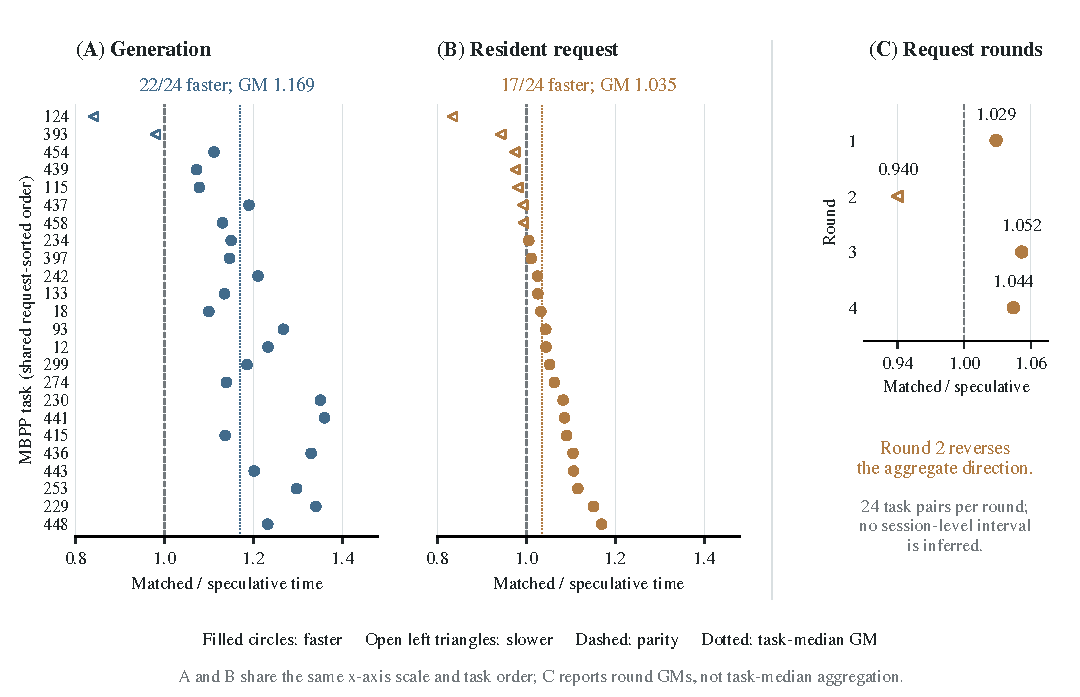
\includegraphics[width=\linewidth]{figures/figure_5_task_variation.pdf}
\caption{Task variation and round sensitivity on the RTX expansion. (A,B) All 24 MBPP tasks, in the same request-sorted order and on the same x-axis scale, use ratios of four-repetition absolute-time medians. Generation improves on 22/24 tasks and request time on 17/24. Filled circles indicate faster speculation and open left triangles slower speculation, independently in each panel; dashed lines mark parity and dotted lines mark the panel geometric means. (C) Request ratios aggregated within each of the four rounds reverse direction in round 2. These round summaries are distinct from the task-median estimator; no session-level uncertainty interval is inferred.}
\label{fig:tasks}
\end{figure*}

Separate resident sessions, laptop scheduling and thermal variation can affect these estimates. Balanced order and task medians reveal some variation but do not remove session confounding. A task bootstrap is not independent session/day replication. We therefore report a qualified positive aggregate operating point, rather than stable production request acceleration. The larger generation gain remains a result for its defined interval, not an end-to-end substitute.

The serial resident-reset study supplies a separate finite check: recorded requests begin with reset target state and the original $k=3$/UB4 recipe retains reference output across two request orders. Its matched generation/request speeds are about $1.181\times/1.039\times$. This supports the registered reset behavior. It is not a concurrency or throughput experiment and is not pooled with the 384 expansion rows.

\subsection{Fixed UB: wider drafting qualifies but becomes slower}
The geometry failures in Section~\ref{sec:repair} change $k$ and UB together. A separate frozen experiment holds UB4 and mask 3 fixed while testing $k=3,5,7$ on 24 now-exposed MBPP inputs plus four exposed HumanEval probes. All widths qualify in two repetitions. The highest passing $k=7$ is selected by qualification alone, then measured in separate capture-off sessions: four conditions, four repetitions and 448 formal requests. Qualification timings are excluded from speed selection.

Relative to the $k=3$ anchor, $k=7$ reaches only $0.829442\times$ generation and $0.889868\times$ resident-request speed. Against matched target-only, it reaches $0.997404\times/0.950353\times$, while the anchor reaches $1.202501\times/1.067970\times$ in that campaign. The widened candidate preserves the reference and fails the extra-cost objective. Ordinary same-width speculation has output failures, so its times remain diagnostic rather than qualified speed evidence.

Formal draft work grows from 3,528 to 5,392 tokens while accepted draft tokens grow from 2,772 to 3,192. In separate captured qualification sessions, target continuation caller calls fall from 305 to 199, but observed micrographs rise from 305 to 397. These sessions include their own warmups and forced synchronization; the counts cannot be combined with formal times into a fabricated per-call profile. Micrographs are not CUDA kernel launches. The evidence rejects caller reduction as a sufficient performance proxy without assigning the slowdown to a unique component.

Saved partitions also matter. At $k=7$, matched generation/request speed is $0.953/0.919\times$ on 24 MBPP inputs but $1.308/1.164\times$ on four HumanEval probes. The pooled result hides these differences. Four exposed probes do not validate a routing rule, and no online selector was developed from them. The supplement retains the longer-cap confirmation and the failed wider-geometry branches without combining their timers into an optimization trajectory.

\subsection{B570: repair improves an old path but loses to strong baselines}
The B570 formal matrix remains 119/120 complete: old N1's first-round MBPP/400 payload is missing after an infrastructure interruption. No request is imputed or rerun in the scientific denominator. Ordinary $R$, matched $M$ and candidate $C$ each have 30 complete responses, providing 15 two-round task-median pairs. Old-N1 comparisons have 14 complete task pairs.

Table~\ref{tab:b570_cost} gives all three timers. Candidate speed is $0.282588\times$ generation and $0.201290\times$ whole request against ordinary $R$, and $0.285761\times/0.205704\times$ against matched target-only. Both baselines are faster in every available paired round. The matched target path is close to ordinary cost ($R/M=0.988893\times/0.978539\times$), so the roughly fivefold candidate request cost cannot be attributed entirely to the consistency constraint on the target path.

% Generated by scripts/reconstruct.py from frozen exports.
\begin{table}[ht]\centering\small
\caption{B570 paid baseline/candidate task-median ratios. $n$ counts complete two-round task pairs: 15 for $R/C$, $M/C$ and $R/M$, and 14 for old N1/$C$. Gen., Request and Host denote generation, whole request and host-observed time. The missing old-N1 task is not imputed; raw suffix work stays charged.}\label{tab:b570_cost}
\setlength{\tabcolsep}{3pt}
\begin{tabular}{@{}lrrrr@{}}\toprule
Ratio & $n$ & Gen. & Request & Host\\\midrule
$R/C$ & 15 & 0.283 & 0.201 & 0.202\\
$M/C$ & 15 & 0.286 & 0.206 & 0.206\\
Old N1/$C$ & 14 & 3.993 & 2.634 & 2.633\\
$R/M$ & 15 & 0.989 & 0.979 & 0.979\\
\bottomrule\end{tabular}

\end{table}


Against old N1, the candidate improves generation/request speed by $3.993091\times/2.633940\times$ over 14 task pairs. That is real engineering progress relative to a slow prior frontend, but does not establish deployment benefit. MBPP/245 also reverses the old-path request comparison in round 2. Neither aggregate improvement nor endpoint recovery supports a universal per-round gain.

The candidate's formal records contain 888 drafted and 702 accepted tokens. Endpoint IDs total 1,150 while raw IDs total 1,176; all 26 suffix IDs remain charged. Target and draft continuation caller-token totals are 1,332 and 1,362. These are distinct runtime quantities. Raw suffix equality is not required by this endpoint contract and is not claimed. Removing witness readbacks, an extra context and handoff improves the frontend, while phase reservation, synchronization, drafting and rollback remain online. No full independent component profile identifies a unique remaining bottleneck. The appropriate decision is to reject this recipe as a latency improvement against the two strong baselines.

\subsection{Global serialization, control, and draft-side limits}
An earlier RTX global-serialization timing arm qualifies 57/57 arrays on 19 exposed tasks but reaches only $0.677351\times$ target-only speed, with descriptive interval approximately $[0.662,0.692]$ and zero tasks faster. Its synchronized post-prefill-to-slot-release interval includes instrumented work and logging, unlike the later server generation field. It is a separate qualified cost failure, not the first point of a common before/after speed curve. The supplement preserves its host-timer amendment and the preceding V3 stop.

M4 addresses control under a separate post-prefill contract (Supplement \S S6.6). A prospective 60-task, three-condition, three-repeat campaign has 540 requests; Always speculation and Guard each qualify 180/180 direct-ID comparisons. Target-only/Always speed is $1.346894\times$, whereas paired secondary Guard/Always latency is $1.027076$ with descriptive interval $[1.012956,1.043559]$. This guard is slower than the fixed policy. A hindsight oracle choosing only target-only or Always leaves about 0.069\% further geometric-mean latency reduction; it does not bound intra-request policies.

On 358H, CPU/NPU drafting each qualifies a 90-request direct-ID panel but reaches only $0.733915\times/0.351663\times$ speed. Holding measured target work and progress fixed, removing all other nonnegative work still gives prompt-estimator ceilings of $0.8372\times/0.8448\times$, below parity. Even this idealization requires a uniform target-work reduction of at least 16.28\%/15.52\% to reach parity. Faster isolated drafting cannot meet that budget; a different target path or state interface is needed. Supplement \S S6.7 gives the conditional derivation, component totals and distinct pooled estimator. Neither M4 nor 358H is a cross-platform replication of the RTX repair.
\FloatBarrier
